\subsection{Cosmic Radiation Methods}
\label{sec:Cosmic-Radiation-Methods}

The Timepix sensors output data in a human-readable, array-like format that directly corresponds to the pixel array of the sensor.
The sensor collects data in a manner similar to that of an optical camera.
A shutter time is a parameter defined by the user, and the sensor will collect data for the entire duration of the shutter time.
Once the time has lapsed, the sensor packages the data into a data frame and is sent to the storage of the computer.
The length of the shutter time must be carefully chosen.
Too short of a length will result in many empty data frames that waste storage space, but too long of a length will result in data frames which are unreadable since the particle tracks in the frame will be indistinguishable from one another.
Each pixel in the 256 by 256 sensor array has one corresponding energy value per frame, so this array can be used to reconstruct the data frame.
The energy threshold is another user-defined parameter that determines the minimum energy which can be detected by the sensor.
The primary purpose of the energy threshold is to filter out extraneous whitenoise from the environment.
<< FINISH THIS: Add the energy threshold and the shutter time used for the devices in the mission >>
An example of a data frame can be seen in Figure \ref{fig:minipix-example-frame}
A separate file contains the metadata for each data frame, and contained within the metadata is information such as the energy threshold and the timestamp.

\begin{figure}[h!]
	\begin{center}
		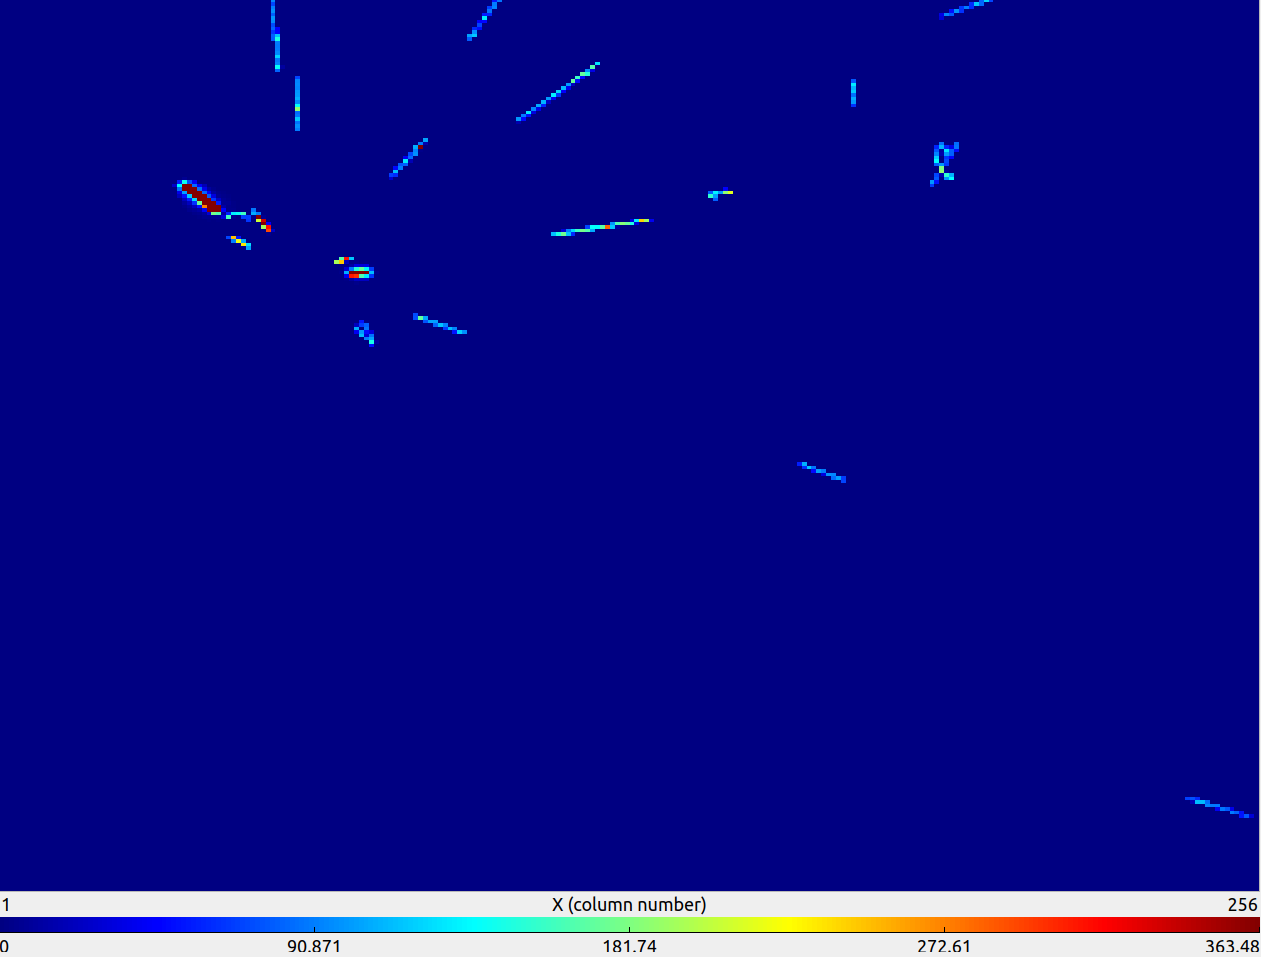
\includegraphics[width=\textwidth]{figures/interesting-frame-3447.png}
		\caption{Example of a Timepix data frame. This is one of the MiniPIX data frames from the 2019 mission.}
		\label{fig:minipix-example-frame}
	\end{center}
\end{figure}

% Detail the analysis techniques used to determine the morphology and the dose (see 2018 report)


\subsection{Organic Solar Cell Methods}
\label{sec:Solar-Cell-Methods}

This is the organic solar cell methods.

